\documentclass[12pt,a4paper]{report}

\usepackage{graphicx}

\usepackage[utf8]{inputenc}
\usepackage[english]{babel}
\renewcommand{\baselinestretch}{1.2} % line spacing

\usepackage{hyperref} % this for hyperlinks

\usepackage[left=3.5cm,right=3cm,top=3cm,bottom=3cm]{geometry}

\usepackage{multirow}
\usepackage{tabu} % for DHTvsDFT table; http://ctan.imsc.res.in/macros/latex/contrib/tabu/tabu.pdf

%\usepackage[framed,numbered,autolinebreaks,useliterate]{mcode} % for matlab code; http://www.howtotex.com/tips-tricks/how-to-include-matlab-code-in-latex-documents/

\usepackage[nottoc,notlot,notlof]{tocbibind} % for references in ToC; http://www.howtotex.com/packages/how-to-add-bibliography-and-more-to-table-of-contents/

%\usepackage[titletoc]{appendix} % Appendix word in ToC; https://tex.stackexchange.com/questions/44858/

\usepackage{mathtools}
\DeclarePairedDelimiter{\ceil}{\lceil}{\rceil} % for ceil sign https://tex.stackexchange.com/questions/42271/floor-and-ceiling-functions

\begin{document}

%\title{}
%
%\author{Emtiaj Hasan}

%\maketitle


%\documentclass[12pt,a4paper]{report}
%\usepackage{blindtext}
%\usepackage{graphicx}
%
%\usepackage{hyperref} % this for link


%\begin{document}

\pagenumbering{roman}

%page 1

\thispagestyle{empty}

\begin{center}
\textbf{{\large Bachelor of Science in Computer Science and Engineering}}

\vspace{75mm}

\textbf{{\large A Zero-Watermarking Scheme Based on Discrete Hartley Transform for Audio Signal} }

\vspace{30mm}

\textbf{Emtiaj Hasan}

\textbf{ID: 1004050}

\vspace{15mm}

\textbf{March, 2016}

\vfill

\textbf{{\large Department of Computer Science \& Engineering} \newline
{\normalsize Chittagong University of Engineering \& Technology} \newline
{\small Chittagong-4349, Bangladesh}}
\end{center}

\newpage

%page 2

\thispagestyle{empty}

\begin{center}
\textbf{{\large A Zero-Watermarking Scheme Based on Discrete Hartley Transform for Audio Signal} }


\includegraphics[scale=.75]{image/cuet-logo.png}


This thesis is submitted in partial fulfillment of the requirement for the degree of Bachelor of Science in Computer Science \& Engineering. \newline

\vspace{10mm}

Emtiaj Hasan

ID: 1004050


\vspace{20mm}

Supervised by \

Dr. Pranab Kumar Dhar \

Assistant Professor \

Department of Computer Science \& Engineering (CSE) \

Chittagong University of Engineering \& Technology (CUET)




\vfill
\textbf{{\large Department of Computer Science \& Engineering} \\
{\normalsize Chittagong University of Engineering \& Technology} \\
{\small Chittagong-4349, Bangladesh}}
\end{center}

\newpage

%page 3

\thispagestyle{empty}

The thesis titled \textbf{\textquotedblleft A Zero-Watermarking Scheme Based on Discrete Hartley Transform for Audio Signal\textquotedblright} submitted by Roll No. 1004050, Session 2013-2014 has been accepted as satisfactory in fulfillment of the requirement for the degree of Bachelor of Science in Computer Science \& Engineering (CSE) as B.Sc. Engineering to be awarded by the Chittagong University of Engineering \& Technology (CUET).

\vspace{20mm}
\begin{center}
{\Large \textbf{Board of Examiners}}
\end{center}

\vspace{10mm} 
\noindent 1. \rule{4cm}{0.4pt} \hfill Chairman  \newline
Dr. Pranab Kumar Dhar \newline
Assistant Professor \newline
Department of Computer Science \& Engineering (CSE) \newline
Chittagong University of Engineering \& Technology (CUET) \newline


\vspace{10mm} 
\noindent 2. \rule{7cm}{0.4pt} \hfill Member  \newline Professor Dr. Mohammed Moshiul Hoque \hfill (Ex-officio) \newline
Head \newline
Department of Computer Science \& Engineering (CSE) \newline
Chittagong University of Engineering \& Technology (CUET) \newline

\vspace{10mm} 
\noindent 3. \rule{3.5cm}{0.4pt} \hfill Member  \newline
Md. Monjur-Ul-Hasan \hfill (External) \newline
Assistant Professor \newline
Department of Computer Science \& Engineering (CSE) \newline
Chittagong University of Engineering \& Technology (CUET) \newline

\newpage


%page 4

\thispagestyle{empty}

\begin{center}
{\Large \textbf{Statement of Originality}}
\end{center}

\vspace{10mm}
It is hereby declared that the contents of this thesis is original and any part of it has not been submitted elsewhere for the award of any degree or diploma.

\vspace{50mm}

%\noindent\rule{6cm}{0.4pt} \hfill \rule{6cm}{0.4pt}
%
%\noindent\textbf{Signature of the Supervisor}	 \hfill \textbf{Signature of the Candidate}	\newline
%\textbf{Date}:  \hspace{77mm} \textbf{Date}: \newline

\noindent\rule{5.7cm}{0.4pt}

\noindent\textbf{Signature of the Candidate} \newline \textbf{Date}:

\newpage

\section*{Acknowledgment}
This thesis gives me an opportunity to thank all of the people who have helped me throughout my graduation life. First of all, I am grateful to my honorable project Supervisor Dr. Pranab Kumar Dhar, Assistant Professor, Department of Computer Science and Engineering, Chittagong University of Engineering and Technology, for the guidance, inspiration and constructive suggestions which were helpful in the preparation of this project. I also convey special thanks and gratitude to Professor Dr. Mohammed Moshiul Hoque, honorable head of the Department of Computer Science and Engineering, Chittagong University of Engineering and Technology, for his kind advice. I would also like to extend my gratitude to all of my teachers for their valuable guidance in every step of my learning stage. I would like to thank my friends for their cooperation that has helped in the successful completion of the project. Special thanks to the staffs of the department for their assistance. Last but not the least, I would like to thank my parents for supporting me throughout my entire life. Without their encouragement, it would not be possible to make this achievement.

\newpage

\section*{Abstract}
Internet is the fastest medium of transferring data to any place in a world and a popular digital media is audio. Various cloud-based storage contains a huge database of digital audio. Moreover, for the cheaper price of different storage device e.g., flash drive, make it easier for people to share, distribution of audio files easily and sometimes illegally. For these reasons, the chances of copyright infringement are higher than ever and measures against piracy were never so demanded. In this view, an audio watermarking field is very important. Considering the growing demand for this field, this thesis proposes a new zero-watermarking scheme based on Discrete Hartley Transform (DHT) for audio signal. In this scheme, DHT is performed on audio and a binary pattern is generated so that it can be used for extraction of the watermark in later. The experimental results show that this algorithm can resist various attacks. In most of the cases, the correlation between the original watermark and the extracted watermark is more than 0.9 and also bit error rate is less than 12\% which demonstrates that the proposed method is a suitable candidate for copyright protection. Furthermore, comparing with other existing schemes, it shows much better robustness against several attacks.

%\end{document}

\tableofcontents

\listoffigures

\listoftables

\chapter{Introduction}

\setcounter{page}{1}
\pagenumbering{arabic}

\section{Digital Watermarking}

This is the era of internet and people from every corner of the world are connected via this. The proliferation of internet gives the opportunities of easy access, sharing, distribution, storage of digital content such as images, video, audio, text. Since data exposed on the Internet is easily accessible to anyone, such media contents are facing serious challenges like piracy, illegal redistribution, forgery, etc. Digital watermarking technology is an effective solution to meet such challenges.

\bigskip

Embedding some kind of information into data for tamper detection, authentication, traitor tracing, etc is known as watermarking. The embedded data is called watermark. In visible digital watermarking, the information is visible in the picture, text or video. In invisible digital watermarking, information is added as digital data to audio, text, picture or video.

\bigskip

Digital watermarking is a procedure of hiding some information into digital multimedia content, possibly in an imperceptible way without degrading the quality of the content. Furthermore, the watermark must be either robust or fragile, depending on the application.A watermark is called fragile if detection fails with even minor modification. It is useful in tempering detection. A watermark is called robust if detection is accurate under any modification. It is used in copyright control application.

\bigskip

Recently, many efforts have been devoted to the problem of copyright protection by plenty of research communities. This is because that multimedia data has become a widely used carrier of information and the rapid growth of internet has made the copyright and integrity of digital media information more and more crucial issues. To protect digital data against illegal use and tampering, digital watermarking has been proposed to accomplish copyright protection or content
integrity authentication.


\subsection{General Concept of Watermarking}

The information to be embedded in a signal is called digital watermark, and the signal where the watermark is to be embedded is called the host signal. A watermarking system is usually divided into three distinct steps: embedding, attack and extraction.

\begin{figure}[h!]
\centering
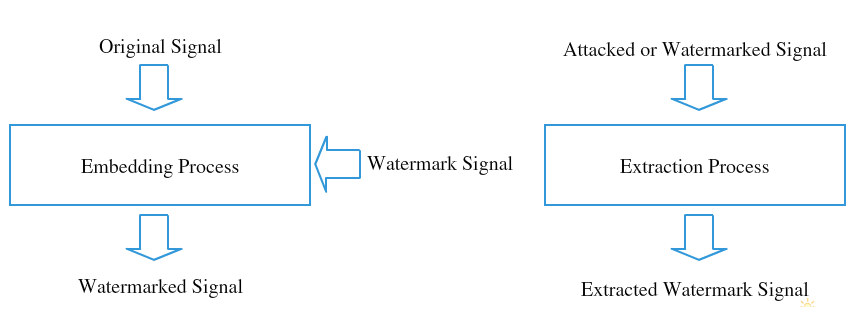
\includegraphics[scale=0.6]{image/WatermakProcess.png}
\caption{Basic structure of watermarking process}
\label{fig:wtrprocess}
\end{figure}

\bigskip

In embedding, an algorithm accepts the host and the data to be embedded and produces a watermarked signal.

\bigskip

Then the watermarked signal is transmitted or stored, usually transmitted to another person. If this person or the medium through which it is transmitted, makes a modification then this is called attack. Some attack may perform on host signal for practical reason, e.g., to consume storage, image or audio or video may be compressed. But the term \textquotedblleft attack\textquotedblright may arise in perspective of sharing data, where man in the middle attempt to remove the digital watermark through modification.

\bigskip

Extraction (also called detection) is an algorithm which is applied to the attacked or watermarked signal to attempt to extract to the watermark from it. If the signal was unmodified during transmission, then the watermark still is present and it may be extracted. In robust digital watermarking, the extraction algorithm should be able to produce the watermark correctly, even if the modifications were strong. In fragile digital watermarking, the extraction algorithm should fail if any change is made to the signal. %A basic structure of watermarking process is illustrated in Fig. \ref{fig:wtrprocess} at page \pageref{fig:wtrprocess}.


\subsection{Classification of Watermarking}

There are many watermarking techniques in terms of their application areas and purposes. And they have different insertion and extraction techniques. 

\bigskip

Watermarking  techniques  can  be  divided  into  four  categories  according  to  the type of document to be watermarked as follows:

\begin{itemize}

\item Text Watermarking
\item Image Watermarking
\item Audio Watermarking
\item Video Watermarking

\end{itemize}

\bigskip

According to human perception watermarking can be categorized as follows:

\begin{itemize}

\item Visible Watermarking, where watermark can be sensed by the human without extraction. For example, logos that are used in papers and videos.

\item Invisible Watermarking, where watermark can be detected by only applying proper extraction algorithm.

\end{itemize}

\bigskip

Watermarking can also be divided into two categories according to the watermark extraction procedures requirement:

\begin{itemize}

\item Blind Watermarking, which do not require host signal to extract the watermark. 

\item Non-blind Watermarking, it needs the original signal to extract the watermark.

\end{itemize}

\bigskip

All watermarking techniques are not equally robust against attacks or manipulations. Based on the level of robustness, watermarks are classified into three categories:

\begin{itemize}

\item Robust Watermarking, it can recover watermark after applying severe attacks.
\item Fragile Watermarking, it fails even on light attacks.
\item Semi-fragile Watermarking, it is better than fragile but not than robust.

\end{itemize}

\bigskip

Based on the key used in embedding and extraction, watermarking techniques can be categorized into two classes:

\begin{itemize}

\item Symmetric Watermarking, here the embedding key and the detection key are same.

\item Asymmetric Watermarking, this technique uses different embedding and detection key. This type of work is clearly more secured than the symmetric type but it also implies higher complexity.

\end{itemize}


\subsection{Properties of Watermark}

For a digital watermark to be effective and practical, it should be exhibit the following properties:

\begin{itemize}

\item \textbf{Imperceptibility}: A digital watermark is called imperceptible if the original signal and the marked signal are perceptually indistinguishable. It is inaudible to human auditory system. It remains hidden in content and can be detected only by authorized agencies. And a digital watermark is called perceptible if its presence in the marked signal is noticeable.

\item \textbf{Security}: The watermarking procedure should rely on secret keys, not the algorithm's secrecy, to ensure security, so that pirates cannot detect or remove watermark. If the key that is used during watermarking is lost or the key is public, the watermark can be read and also be removed.

\item \textbf{Robustness}: It is not possible for a watermarking scheme to be robust against all possible signal processing operations. Practically no perfect method is proposed so far that can withstand against all kinds of attacks. But a robust watermark should be able to withstand the basic operation.

\end{itemize}

\subsection{Application of Watermarking}

\begin{itemize}

\item \textbf{Copyright Protection}: A person should embed watermark into host signal to protect against illegal distribution. Suppose, person A creates an image and embeds watermark into it. He sends it to person B for some reason. If person B tries to sell it to others without the permission of person A, then person A can extract his watermark and proves his ownership.

\item \textbf{Source Tracking}: Different recipients get differently watermarked content so that no one can distribute to other. For example, watermark is embedded into each movie's DVD. If the movie is then leaked to the internet, the movie producers could identify which recipient of the movie was the source of the leak.

\item \textbf{Broadcast Monitoring}: Advertising agencies want to ensure their commercials are properly aired, as they want this commercial to be displayed at the exact time they wanted to. In this thing, watermark is applied. Information that can identify the individual video, embedded to video using watermarking, making broadcasting easier.

\item \textbf{Fingerprinting}: The main purpose of fingerprinting is to protect customers. If someone got a legal copy of a product but redistributed illegally, fingerprinting can prevent this. This can be achieved
by tracing the whole transaction by embedding unique robust watermark for each recipient. Thus, the owner can identify who redistributed this product by extracting the
watermark from the illegal copy.

\item \textbf{Indexing}: Comments and markers or key information related to the data are inserted as watermark. This watermark information is used by a search engine for retrieving the required data quickly and without any ambiguity.

\item \textbf{Meta-data Tagging}: Watermarks convey object specific information to user of the object. For example, it is used to attach patient identification data to medical images.

\end{itemize}

\section{Motivation}

In recent years, the increasing amount of applications using digital multimedia technologies has emphasized the need to protect digital multimedia data from piracy. Authentication and information hiding, copyright protection, content identification, proof of ownership has also become important issue. Hence watermarking is becoming more and more important. Therefore, digital watermarking technique has received a great deal of attention recently in the literature and among the research community, but currently, most of the digital watermarking schemes mainly focus on image and video copyright protection. Digital audio watermarking technology provides a special challenge because the human auditory system is extremely more sensitive than the human visual system. Furthermore, audio signal contains
one-dimensional data, thus it is difficult to hide additional information without compromising the quality of the audio signal. That is why audio watermarking is chosen for thesis work. To propose a watermarking method that will be robust and imperceptible to be a strong contestant of currently available audio watermarking methods for copyright protection of audio content is the motivation.


%\section{Prospect of the Proposed Watermarking \\ Scheme}
\section{Prospect of the Proposed Watermarking Scheme}


\begin{itemize}

\item 
To develop a watermarking scheme based on Discrete Hartley Transform.

\item
To develop a blind audio watermarking algorithm.

\item
To develop an imperceptible and robust audio watermarking algorithm.

\end{itemize}


\section{Organization of the Thesis}

This thesis is divided into six chapters. This chapter briefly discussed a general watermarking scheme and its properties and application areas. In addition, the motivation and objectives of this thesis are presented. The remaining of this thesis is organized as follows:

\bigskip

In chapter 2, description about the previous research that have been done on audio watermarking is included. Chapter 3 presents the methodology of the proposed watermarking scheme, including watermarking embedding process and watermarking extraction process. Chapter 4 contains the detail description of the implementation procedures of the proposed watermarking scheme. Chapter 5 includes the simulation results and the performance  evaluation of the proposed system in terms of robustness, imperceptibility and other properties. Chapter 6 concludes the thesis with mentioning the goal achieved by this research work.


\chapter{Literature Review}

\section{Audio Watermarking}
Since the internet rapidly grows, networks carry
large amounts of multimedia data. But the blessings of internet help unethical or bad people to reproduce unauthorized copies and illegally distribute these copies without the consent of the owner. To prevent this, the audio watermarking field is very important. By definition, audio watermarking is the technique of embedding of owner copyright identification into the host audio.

\section{Audio Watermarking Techniques}

A significant number of audio watermarking techniques have been reported in recent years in order to create robust and imperceptible audio watermarks. Audio watermarking techniques that proposed so far can be divided into various groups, such as, time domain, transform domain, zero-watermarking technique.

\subsection{Time Domain Method}

Time domain based methods embed watermark information into the time domain. These methods are simple and easy to implement and most of them can retrieve watermark
without referencing the original audio. The main disadvantage of time domain based schemes is its immunity to manipulations. Two main methods belonging to this category are least significant bit (LSB) based method and echo hiding based method. 

\bigskip

The simplest time domain based watermarking is least significant bit \cite{zhang} method which simply uses the least significant bits of the host audio signal to embed
watermark data. A moderately robust time domain based spread spectrum technique was proposed by Bassia \cite{bassia}. Foote \cite{foote} proposed a non-blind watermarking scheme using time based modulation. Lie \cite{wnlie} proposed another time domain based watermarking scheme where they used differential average of absolute amplitude relations within each group of samples to represent one bit information. To preserve the time domain waveform envelope they employed low frequency amplitude modification to scale amplitudes in a group manner in selected sections of samples. Lemma \cite{lemma} proposed modified audio signal keying (MASK) to modify the short time envelope of the audio signal in an imperceptible approach.

\bigskip

Echo hiding based watermarking techniques embed the watermark by introducing an echo. However, echo hiding can effectively embed watermarks in imperceptible way \cite{hooh}, \cite{kbyeong} but in such schemes watermark can be easily detected by anyone.

\subsection{Transform Domain Method}

In transform domain watermarking techniques, an audio is processed by means of a specific transform. Transform domain based watermarking techniques have been proven to be much more effective with regard to accomplishing the imperceptibility and robustness requirements of digital watermarking algorithms. The frequency domains such as Discrete Cosine Transform (DCT), Discrete Wavelet Transform (DWT) and Discrete Fourier Transform (DFT) are more specifically to be dealing with audio watermarking system.

\bigskip

The DFT is a well known and powerful computational tool for performing frequency analysis of discrete time signals. Fast Fourier Transform (FFT) is an efficient algorithm for calculating DFT. It takes a discrete signal in the time domain and transforms the signal into the discrete frequency domain.

\bigskip

A novel time domain synchronization technique \cite{david} was proposed together with a new blind watermarking scheme which works in the DFT domain. Fallahpour \cite{fallahpour} proposed a novel high-capacity audio watermarking system to embed data and extract them in a bit-exact manner by changing some of the magnitudes of the DFT spectrum. Another computationally less complex DFT domain based audio watermarking scheme using quantization was proposed \cite{wtan}. In addition those, various number of audio watermarking methods utilizing DFT have been proposed. Most methods embed watermark information into the magnitude of the DFT components.

\bigskip

The main idea behind the watermarking methods based on DWT is to segment the original audio signal into many frames first and then embed watermark bits into the low or high frequency DWT coefficients.

\bigskip

A blind audio watermarking in DWT domain was proposed by Meng \cite{meng}. To enhance the robustness Chen\cite{stchen} embedded the watermark in the lowest frequency coefficients in DWT domain. Another method was also proposed by same author \cite{stchen2}. Pooyan \cite{pooyan} introduced an audio watermarking system which embeds watermarks in wavelet domain. The watermarks are embedded into the low frequency coefficients in discrete multiwavelet transform domain by Kumsawat \cite{kumsawat2008digital} to achieve robust performance against common signal processing procedures and noise corruptions.

\bigskip

Zeng \cite{zeng} described a blind watermarking system which embeds watermarks into DCT coefficients by utilizing quantization index modulation technique. In \cite{pranab}, authors proposed a method based on DCT for copyright protection. Guo \cite{guo} proposed DCT domain based audio signal watermarking. A watermark algorithm based on DCT and audio feature quantization was also proposed \cite{quan2012audio}.

\bigskip

Yong \cite{wang2010audio} proposed an audio watermarking scheme based on the dyadic wavelet transform. The combination of various transformations are also used in audio watermarking, e.g., combination of DWT and DCT \cite{ji2011quantified}, combination of DWT and DCT with Singular Value Composition (SVD) \cite{dhar2013dwt}, combination of Lifting Wavelet Transform and Singular Value Decomposition \cite{lei2012robust}, have been proposed.

\subsection{Zero Watermarking Method}

In the watermarking schemes previously mentioned, the insertion of watermark into the original signal inevitably introduces some perceptible quality degradation. Another problem is the inherent conflict between imperceptibility and robustness. Zero watermarking technique can solve these problems successfully.

\bigskip

Zero-watermarking does not modify the original signal but constructs zero watermarks from it. Instead of embedding watermark into the host signal, the zero-watermarking approach just constructs a pattern based on the essential characteristics of the host signal and uses them for watermark recovery.

\bigskip

A zero-watermark algorithm was applied by Wen Quan \cite{sun2002zero}, \cite{wen2003concept} for the first time for image authentication. In recent, the audio zero-watermarking scheme has acquired the considerable progress. A zero-watermarking scheme has been proposed to analyze the security of audio signals \cite{zws} presented a method for mapping the approximate coefficients of the wavelet transform of an audio segment into a binary matrix. A zero-watermarking algorithm, based on the Discrete Wavelet Transform (DWT), has been used to construct secrete keys \cite{bzwdwt}, \cite{dwt}. By using the audio's statistical character, \cite{bzwdwt} consults the mean of the approximation coefficients of a one dimensional signal and constructs the watermark sequence with the zero-watermark scheme. Since most of the audio's energy is concentrated at the lower frequency coefficient sets and therefore embedding watermarks in these coefficient sets may degrade the audio significantly, therefore, in \cite{dwt}, to increse robustness, watermark is embedded in the low frequency coefficient sets. Xueying \cite{zhang2014robust} proposed a robust audio zero-watermarking algorithm which extracts the low frequency components of original audio to construct zero-watermarking by using the wavelet packet analysis method. Discrete Wavelet Transform (DWT) and Discrete Cosine Transformation (DCT) have been combined to generate the watermarking sequences \cite{ieee}, \cite{eurasip}. The multiresolution characteristic of discrete wavelet transform (DWT), the energy compression characteristic of discrete cosine transform (DCT) and the steady sign of certain DWT-DCT coefficients are combined in these two scheme. Howevere, the Gaussian noise suppression property of higher order cumulant are also combined with DWT-DCT in \cite{eurasip}. Ciptasari \cite{ciptasari2011efficient} proposed a modified version of \cite{eurasip} by producing a secret key rather than three secret key. An audio zero-watermarking algorithm \cite{zernik} has been proposed which combined DCT with zernike moments. The reason of using zernike moment is the characteristic of non sensitivity to noise of zernike moment. Based on the correlation of Linear Prediction Cepstrum Coefficients (LPCC) with adaptive factors, a zero-watermarking audio scheme has been proposed \cite{yclu}. By calculating the bi-level characteristic sequence of audio signal through the Modified Discrete Cosine Transform (MDCT), a zero-watermark of audio is proposed by \cite{mlwang}. Coupled with bi-level watermark image and the secrete key this scheme show robustness against various attack. The concept of the zero-watermark based on LPCC with a weighting function was proposed to protect audio signals \cite{smtsai}, \cite{lpcc}	. Using the correlation of LPCC with weighted factor, those can retrieve the available embedded watermark back after various attacks. Zero-watermark based on energy was also proposed to protect audio signals \cite{energy}. This scheme calculates the energy of each frame after segmenting the audio. The characteristic of energy is utilized to retrieve the watermark after various attacks.

%Here, an audio watermarking approach based on Discrete Hartley Transform, which is zero watermarking technique, is proposed. Experimental results demonstrate that the proposed technique outperforms the existing audio watermarking techniques against various attacks.


\chapter{Proposed Audio Watermarking Scheme}

From the previous chapter, it can be seen that several audio watermarking schemes have been proposed. As there is no need to embed the watermark in the zero-watermarking method, it can remove the contradiction between robustness and imperceptibility. Though various zero-watermarking schemes exist for the audio signal, still there is a need to work on this method. The main problem is, for some signal processing manipulation i.e., compression, adding echo, re-sampling, etc, existing schemes do not perform satisfactory result. To overcome the limitation, here, this thesis proposes a new zero-watermarking scheme based on discrete Hartley transform.

\section{Background Information}

Discrete Fourier transform (DFT) plays a vital role in signal processing. Despite its tremendous application, the DFT has an unattractive feature, that, it transforms a real-valued sequence also into a complex-valued sequence. R. N. Bracewell \cite{rnb} proposed an inherently real-valued transform called the Discrete Hartley transform (DHT). The new transform has the advantage that a real-valued signal always generates a real-valued transform signal. Also, unlike the DFT, the DHT is symmetric i.e., both the forward and inverse transforms are identical. Moreover, for computing real sequence, Fast Hartley Transform (FHT) is faster than Fast Fourier Transform (FFT) \cite{faster}. Table \ref{table:ftht} gives the comparative analysis between DFT and DHT.

\begin{table}[h!]
 \centering
\begin{tabu} to \linewidth {|X|X|}
 \hline
 \rowfont [c]{\bf } DFT & DHT \\ % center & bold
 \hline
 It has complex values in the transform equation. & It has only real values in the transform equation. \\
 \hline
 The forward and inverse transforms are non-identical. & The forward and inverse transforms are identical. \\
 \hline
 It needs to keep track of +i and -i terms. & No such requirement. \\
 \hline
 Computational complexity is higher due to imaginary terms. & Computational complexity is lower as compared to its counterpart.\\
 \hline
 \end{tabu}
 \newline
 \caption{Comparison of DFT and DHT}
 \label{table:ftht}
\end{table}

\newpage

Considering a sequence of $N$ real numbers $ x_{n} $ for $ n = 0, 1, ..., N-1 $, the DHT of this sequence is defined by equation \ref{eq:dht}.

\begin{equation} \label{eq:dht}
H_{k} = \sum_{n=0}^{N-1} x_{n}[\cos(\frac{2\pi nk}{N}) + \sin(\frac{2\pi nk}{N})]
\end{equation} 

\begin{center}
$ k = 0, 1, ..., N-1 $
\end{center}


\section{Proposed Method Based on Discrete Hartley Transform}

The proposed scheme is divided into three parts. These are watermark embedding process, applying attack and watermark extraction process. Firstly, in embedding process, a key to extract watermark is generated by using the properties of audio. After that, different types of attacks are applied to the audio and then, watermark is extracted from the attacked audio.

\bigskip

Let $ A = \lbrace a(i); i = 1,2,...,L\rbrace $ be the host audio signal and $ W = \{w(i,j); i=1,2,...,M_{1}, j=1,2,...,M_{2}\} $ be the binary-valued image watermark to be embedded.

\subsection{Watermark Embedding Process}

The watermark embedding procedure shown in Fig. \ref{fig:embedding} at page \pageref{fig:embedding} can be described as follows:

\begin{figure}[h!]
\centering
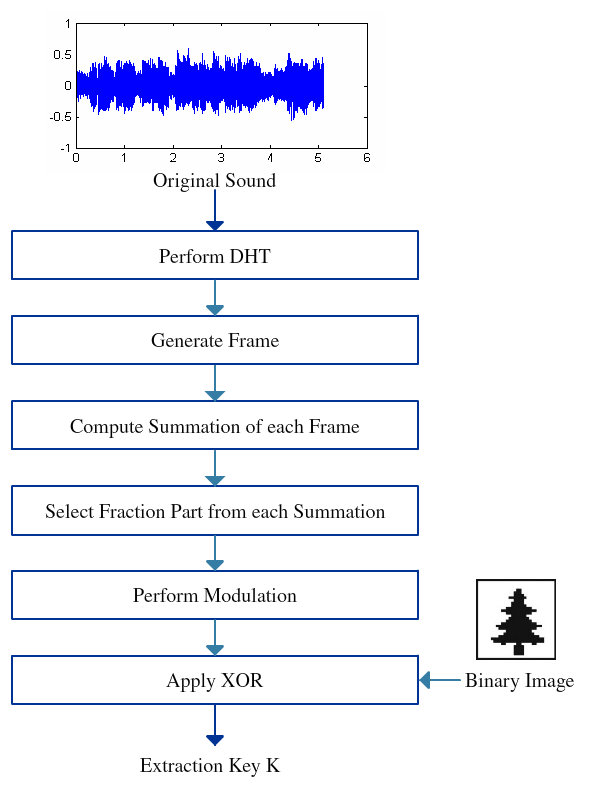
\includegraphics[scale=.7]{image/Embedding.png}
\caption{Watermark embedding process of the proposed scheme}
\label{fig:embedding}
\end{figure}

\bigskip

Step 1:
The discrete Hartley transform is applied to the audio $ A $, and can get the coefficient $ C = \lbrace c(i); i = 1,2,...,C_{A} \rbrace $, which has $C_{A}$ samples.

\bigskip

Step 2:
$ C $ is segmented into $ M $ frames, each frame includes $Q$ samples.

\bigskip

Step 3:
for $i=1:M$

\bigskip

\hspace{10mm}3.1) Compute $s_{i}=\sum_{n=1}^{Q} |C_{n}|$; where $|C_{n}|$ means absolute value of $C_{n}$.

\bigskip

\hspace{10mm}3.2) Compute $ t_{i} = convert( s_{i} - floor(s_{i}) ); $ where $ floor(s_{i}); $ is a function which gives the largest integer less than or equal to $ s_{i} $, in a word, a function which extract integer part from a real value, and $ convert(); $ is a function which converts a fractional value into an integer value.

\bigskip

\hspace{10mm}3.3) Compute $ x_{i} =  mod(t_i^p,2); $ where $p$ is the $t_{i}$ th prime. %Here, if we consider previous example, as $24$th prime is $89$, so two parameter of modulus operation are $24^{89}$ and $2$ respectively.

\bigskip

Step 4:
Convert $x$ into $M_{1}XM_{2}$ matrix.

\bigskip

Step 5:
Compute the watermarking extraction secret key $ k(i,j) $ by doing the exclusive or operation between $w(i,j)$ and $x(i,j)$. Therefore, $ k(i,j) = w(i,j) \oplus x(i,j). $

\bigskip

Here, in step 3.2, the output value is the fractional part of the value found from previous step i.e., 3.1. Suppose after calculation of step 3.1, the summation value is 13.24. In that case, the output of step 3.2 is 24. And about step 3.3, here, considering previous example, as 24th prime is 89, the two parameter of modulus operation are $ 24^{89} $ and $ 2 $ respectively.

\subsection{Attacks on the Host Audio}

In watermarking terminology, an \textquotedblleft attack\textquotedblright is any process that may impair detection of the watermark or the information conveyed by the watermark. It can be classified as:

\begin{itemize}

\item Intentional attack, which is an attempt to weaken, remove or the alter the watermark or original sound.

\item Non-intentional attack, which can occur during audio processing and are not aimed at tempering. For example, lossy compression of audio such as, mp3 audio compression.

\end{itemize}

Different types of attack are described below:

\begin{enumerate}

\item \textbf{Additive Noise}: In audio, noise is generally any unpleasant sound and more technically, any unwanted sound that is unintentionally added to a sound. In digital recording sound, noise is often present. When doing digital recording, the conversion of a sound file from 16 bit to 8 bit adds a layer of noise. Noise may originate from Digital to Analog (DAC) and Analog to Digital (ADC) conversion or as a consequence of transmission error. %White noise is a sound that contains every frequency within the range of human hearing (generally from 20 hertz to 20 kHz ) in equal amounts. Additive white Gaussian noise (AWGN) is a basic noise model used in information theory to mimic the effect of many random processes that occur in nature. Here additive means, noise is added to a signal. White refers to the idea that it has uniform power across the frequency band for the information system. It is an analogy to the color white which has uniform emissions at all frequencies in the visible spectrum. And Gaussian because it has a normal distribution in the time domain with an average time domain value of zero.

\item \textbf{Re-sampling}: Re-sampling or sample rate conversion is the process of changing the sampling rate of a discrete signal to obtain a new discrete representation of the underlying signal. Compact Disc Digital Audio and Digital Audio Tape systems use different sampling rates, 44.1 kHz and 48 kHz respectively. Sample rate conversion prevents changes in speed and pitch that would otherwise occur when transferring recorded material between such systems. %If a sample is re-sampled at a lower rate, sample points are removed from the sound file decreasing its size, but also decreasing its available frequency range. When re-sampling to a higher sample rate, extra sample points in the sound file are interpolated. This increases the size of the sound file but does not increase the quality.

\item \textbf{Filtering}: %Any medium through which the audio signal passes, whatever its form, can be regarded as a filter. However, a filter is not called a filter unless it can modify the sound in some way. 
A digital filter is a filter that operates on digital signals, such as sound. It is a computation which takes one sequence of numbers and produces a new sequence of numbers. Being a frequency dependent amplifier, in its most basic form, an audio filter is designed to amplify, pass or attenuate (negative amplification) some frequency ranges. Common types include low-pass filters, which pass through frequencies below their cut-off frequencies, and progressively attenuates frequencies above the cut-off frequency. %A high-pass filter does the opposite, passing high frequencies above the cut-off frequency, and progressively attenuating frequencies below the cut-off frequency.

\item \textbf{Quantization}: Quantization is the process of converting a continuous analog audio signal to a digital signal with discrete numerical values. In a compact disc, an analog recording is converted to a digital signal quantized with 16 bits of data per sample. During this process of conversion, quantization also achieves a tremendous deal of compression, because an analog sample is considered as having infinite resolution, thus requiring an infinite number of bits to represent, while a digital sample is of limited resolution and is represent using a limited number of bits. %This conversion also means that a tremendous amount of information is lost forever. This loss of information might be a serious concern, but can be made imperceptible or tolerable by properly designing the quantization process. If something irrelevance get happened during this process, it can be removed by re-quantizing the already quantized digital signal.

\item \textbf{Echo}: In audio signal processing, an echo is a reflection of sound, arriving at the listener some time after the direct sound. Typical examples are the echo produced by the bottom of a well, by a building, or by the walls of an enclosed room and an empty room. To simulate the effect of echo, one or several delayed signals are added to the original signal. To be perceived as echo, the delay has to be of order 35 milliseconds or above. %Short of actually playing a sound in the desired environment, the effect of echo can be implemented using either digital or analog methods.

\item \textbf{Compression}: Compression is an attack which reduces the size of the original audio for the purpose of reducing the storage. MPEG-1 or MPEG-2 audio layer III, more commonly referred to as mp3, is an audio coding format for digital audio which uses a form of lossy data compression. %When performing lossy audio encoding, that means creating a mp3 file, there is a trade-off between the amount of space used and the sound quality of the result. Typically, the creator is allowed to set a bit rate, which specifies how many kilo bits the file may use per second of audio. The higher the bit rate, the larger the compressed file will be, and, generally, the closer it will sound to the original file.


\end{enumerate}


\subsection{Watermark Extraction Process}

The watermark recovery procedure shown in Fig. \ref{fig:extraction} at page \pageref{fig:extraction} can be carried out as follows:

\begin{figure}[h!]
\centering
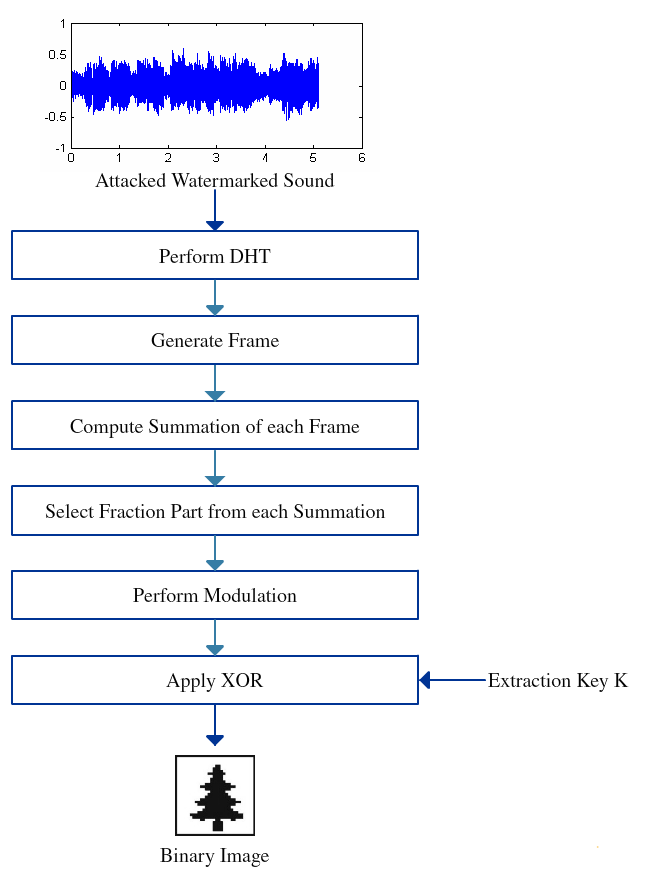
\includegraphics[scale=.7]{image/Extraction.png}
\caption{Watermark extraction process of the proposed scheme}
\label{fig:extraction}
\end{figure}

\bigskip

Step 1:
The discrete Hartley transformation is applied to the watermarked audio $ A^* $, and can get the coefficient 
$ C^* = \{c^*(i); i = 1,2,...,C_A^*\} $, which has $ C_A^* $ samples.

\bigskip

Step 2:
$ C^* $ is segmented into $M$ frames, each frame includes $Q$ samples.

\bigskip

Step 3:
for $i=1:M$

\bigskip

\hspace{10mm}3.1) Compute $s_i^*=\sum_{n=1}^{Q} |C_n^* |$

\bigskip

\hspace{10mm}3.2) Compute $ t_i^* = convert( s_i^* - floor(s_i^*) ); $

\bigskip

\hspace{10mm}3.3) Compute $ x_{i}^{*} = mod(t_{i}^{*p},2);$ where $p$ is the $t_i^*$ th prime.

\bigskip

Step 4:
Convert $ x^* $ into $M_{1}XM_{2}$ size matrix.

\bigskip

Step 5:
Compute the watermarking information $ W^*(i,j) $ by doing the exclusive or operation between $k(i,j)$ and $x^*(i,j)$. Therefore, $ W^*(i,j) = k(i,j) \oplus x^*(i,j). $


\chapter{Implementation of the Project Work}

\section{Audio Files Used for Simulation}

For evaluation the performance of the proposed watermarking method different types audio signals are used. The sound files are: (a) Citizen, Go Back to Sleep, (b) Beginning of the End, (c) Breathing on Another Planet, and (d) Thousand Yard Stare, included in the album \textit{Rust} \cite{rust}. All audio files are 95 seconds long, sampled at 44.1 kHz with 16 bits per sample as shown in Fig. \ref{fig:sample} at page \pageref{fig:sample} . Each audio file contains 4194304 samples. The frame length was fixed at 4096 samples.

\begin{figure}[h!]
\centering
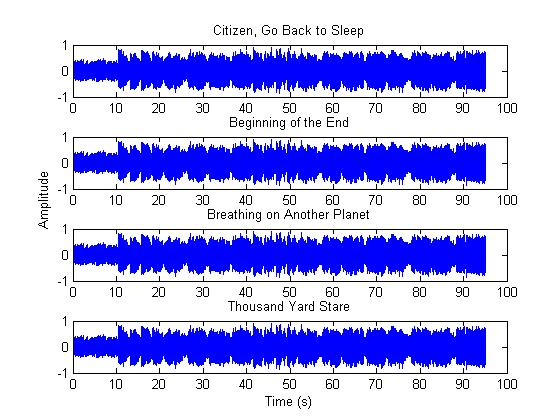
\includegraphics[scale=.8]{image/sample.jpg}
\caption{The signal of original audio}
\label{fig:sample}
\end{figure}


\section{Image Used for Simulation}

In this experiment, a binary image with size 32X32 is used as the watermark shown in Fig. \ref{fig:H} at page \pageref{fig:H}. Image has taken from \cite{bhat2011audio}.


\begin{figure}[h!]
\centering
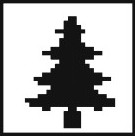
\includegraphics[scale=.8]{image/BN.jpg}
\caption{Watermark image with size 32X32}
\label{fig:H}
\end{figure}


\section{Attacks Applied in Simulation}

In order to test the robustness of the proposed method,
nine different types of attacks are as following:

\begin{enumerate}

\item Noise addition: 20 dB additive white Gaussian noise (AWGN) is added to the audio signal.

\item Re-sampling: The audio signal originally
sampled at 44.1 kHz, is re-sampled at 22.050 kHz, and then restored by sampling again at 44.1 kHz.

\item Low-pass filtering: Adopt a six order Butterworth
filter with cut-off frequencies 11.025 kHz.

\item Re-quantization: The 16 bit audio signal is quantized down to 8 bits per sample and again re-quantized back to 16 bits per sample.

\item Echo: An echo signal with a delay of 0.5s is added to the audio signal.

\item Reverse: The audio is reversed to its original.

\item MP3 compression: MPEG-1 layer 3 compression is applied. The audio signal is compressed at a bit rate of 32 kbps.

\item MP3 compression: MPEG-1 layer 3 compression is applied. The audio signal is compressed at a bit rate of 64 kbps.

\item MP3 compression: MPEG-1 layer 3 compression is applied. The audio signal is compressed at a bit rate of 128 kbps.

\end{enumerate}

GoldWave \cite{goldwave} was used in this experiment for above mentioned attacks except  the AWGN and the re-quantization. Those were implemented using MATLAB \cite{matlab}.

\bigskip

The original sound and attacked sound for sound file \textit{Beginning of the End} are plotted in Fig. \ref{fig:original}, Fig. \ref{fig:noise}, Fig. \ref{fig:resampling}, Fig. \ref{fig:lpf}, Fig. \ref{fig:requantized}, Fig. \ref{fig:echo}, Fig. \ref{fig:reverse}, Fig. \ref{fig:mp332}, Fig. \ref{fig:mp364}, Fig. \ref{fig:mp3128} respectively.

\begin{figure}[h!]
\centering
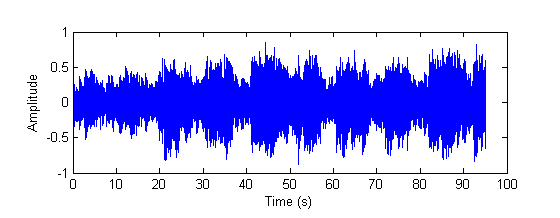
\includegraphics[scale=0.8]{image/original}
\caption{Original audio signal}
\label{fig:original}
\end{figure}

\begin{figure}[h!]
\centering
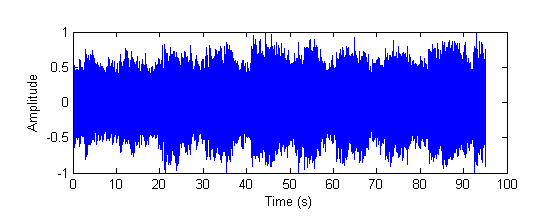
\includegraphics[scale=0.8]{image/awgn.png}
\caption{Audio signal after Gaussian noise adding}
\label{fig:noise}
\end{figure}

\newpage

\begin{figure}[h!]
\centering
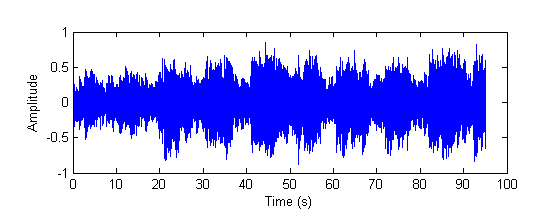
\includegraphics[scale=0.8]{image/resampling.png}
\caption{Audio signal after re-sampling}
\label{fig:resampling}
\end{figure}

\begin{figure}[h!]
\centering
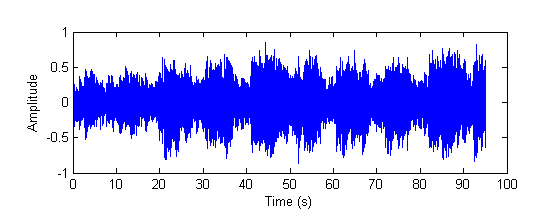
\includegraphics[scale=0.8]{image/lpf.png}
\caption{Audio signal after low-pass filtering}
\label{fig:lpf}
\end{figure}

\begin{figure}[h!]
\centering
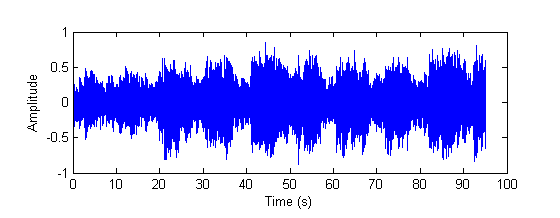
\includegraphics[scale=0.8]{image/requantized.png}
\caption{Audio signal after re-quantization}
\label{fig:requantized}
\end{figure}

\newpage

\begin{figure}[h!]
\centering
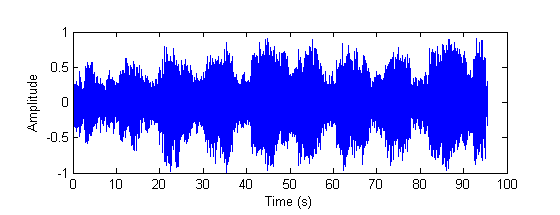
\includegraphics[scale=0.8]{image/echo.png}
\caption{Audio signal after adding echo}
\label{fig:echo}
\end{figure}

\begin{figure}[h!]
\centering
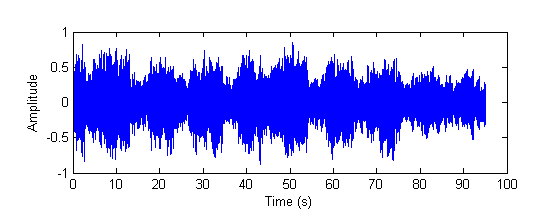
\includegraphics[scale=0.8]{image/reverse.png}
\caption{Audio signal after doing reverse}
\label{fig:reverse}
\end{figure}

\begin{figure}[h!]
\centering
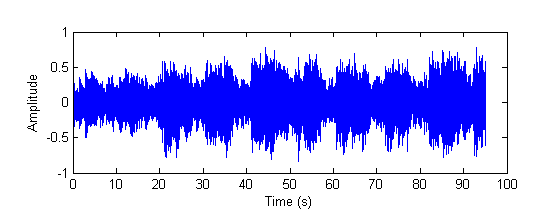
\includegraphics[scale=0.8]{image/mp332.png}
\caption{Audio signal after compressed to mp3/32kbps format}
\label{fig:mp332}
\end{figure}

\newpage

\begin{figure}[h!]
\centering
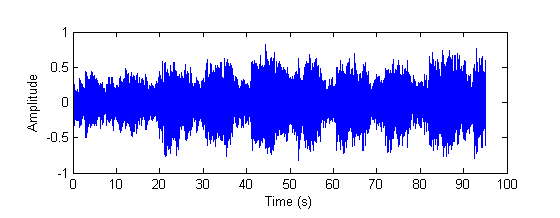
\includegraphics[scale=0.8]{image/mp364.png}
\caption{Audio signal after compressed to mp3/64kbps format}
\label{fig:mp364}
\end{figure}

\begin{figure}[h!]
\centering
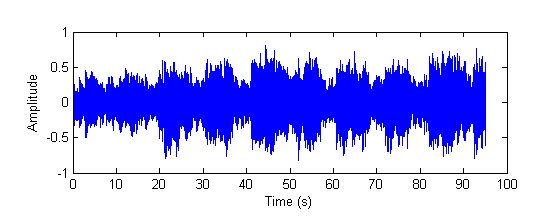
\includegraphics[scale=0.8]{image/mp3128.png}
\caption{Audio signal after compressed to mp3/128kbps format}
\label{fig:mp3128}
\end{figure}

\section{Experimental Environment}

\begin{itemize}
\item \textbf{Processing Software}: MATLAB
\item \textbf{Software for Applying Attack}: GoldWave
\end{itemize}

\section{Normalized Coefficient}

Normalized coefficient (NC) is used to evaluate the similarity between the original watermark and the extracted watermark. In order to evaluate the value of NC, the extracted watermark $W^*$ is compared with the original watermark $W$ and the NC is defined by equation \ref{eq:nc}.

\bigskip

\begin{equation} \label{eq:nc}
NC(W,W^*) = \frac{ \sum_{i=1}^{M_{1}} \sum_{j=1}^{M_{2}} W(i,j)W^*(i,j) } { \sqrt{\sum_{i=1}^{M_{1}} \sum_{j=1}^{M_{2}} W(i,j)^2} \sqrt{\sum_{i=1}^{M_{1}} \sum_{j=1}^{M_{2}} W^*(i,j)^2} }
\end{equation}

\bigskip

where $W(i,j)$ and $W^*(i,j)$ are the original watermark and extracted watermark respectively.

\section{Bit Error Rate}

Bit error rate (BER) is used to evaluate the watermark detection accuracy after signal processing operations and a value of zero or very close to zero is required for good robustness. In order to evaluate the BER, the extracted watermark $W^*$ is compared with the original watermark $W$ and the BER is defined by equation \ref{eq:ber}.

\bigskip

\begin{equation} \label{eq:ber}
BER(W,W^*) = \frac{ \sum_{i=1}^{M_{1}} \sum_{j=1}^{M_{2}} |W(i,j) - W^*(i,j)| } { M_1 X M_2 } X 100\%
\end{equation}

\bigskip

where $W(i,j)$ and $W^*(i,j)$ are the original watermark and extracted watermark respectively, and $M_{1}XM_{2}$ is the size of watermark image. In general, BER is expressed in terms of percentage.

\section{False Positive Error}

False positive error is the probability of declaring an non-watermarked audio as watermarked by decoder. The watermarking system is better with less false alarm probability. Let $k$ be the total number of watermark bits, and $t$ the number of matching bits. The false positive error probability $ P_{fp} $ can be calculated by equation \ref{eq:falsepos}.

\bigskip

\begin{large}
\begin{equation} \label{eq:falsepos}
P_{fp} = 2^{-k} \sum_{t=\ceil{0.8k}}^{k} C(k,t)
\end{equation}
\end{large}

\bigskip

where $C(k,t$) is the binomial coefficient.

\section{False Negative Error}

False negative error is the probability of declaring a watermarked audio as non-watermarked by decoder. The watermarking system is better with less false rejection probability. Let $k$ be the total number of watermark bits, and $t$ the number of matching bits. The false negative error probability $ P_{fn} $ can be calculated by equation \ref{eq:falseneg}.

\bigskip

\begin{large}
\begin{equation} \label{eq:falseneg}
P_{fn} = \sum_{t=0}^{\ceil{0.8k}-1} [C(k,t)p^{t}(1-p)^{k-t}]
\end{equation}
\end{large}

\bigskip

where $C(k,t)$ is the binomial coefficient and $p$ is the bit error probability of extracted watermark. Corresponding to different attack, $p$ has different value. However, the approximate value of $p$ may be obtained from bit error rate under determinate attack.

\chapter{Simulation Result}

\section{Imperceptibility Analysis}

The watermarked audio is identical to original one because the watermark is, actually, embedded into the secret key, not into the audio. So without processing with various imperceptibility analysis methods, it is said to be an imperceptible scheme.

\begin{figure}[h!]
\centering
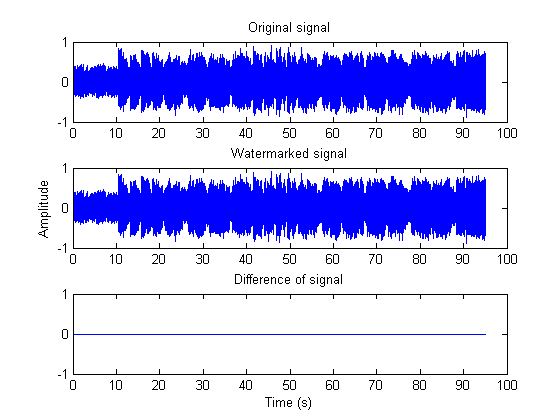
\includegraphics[scale=.8]{image/imperceptibility.png}
\caption{Imperceptibility of proposed watermarking scheme}
\label{fig:imperceptibility}
\end{figure}

\newpage

Fig. \ref{fig:imperceptibility} shows the imperceptibility of the proposed audio watermarking scheme. Here, it is observed that there is no difference between original audio and watermarked audio, which is the proof of its imperceptibility.

\section{Measuring the Robustness}

The robustness of a watermarking method is defined as the ability of watermark detector to extract the embedded watermark after common signal processing and attacks. Robustness is measured in terms of normalized coefficient and bit error rate as described earlier. In order to test the robustness of the proposed scheme, various types of attack are applied mentioned in chapter 4. In the following, the robustness of the proposed scheme against these types of attacks are demonstrate. 

\bigskip

Tables \ref{table:soundone} and \ref{table:soundtwo} show the robustness result of audios (a) \textit{Citizen, Go Back to Sleep}, (b) \textit{Beginning of the End}, (c) \textit{Breathing on Another Planet} and (d) \textit{Thousand Yard Stare} respectively. In table \ref{table:soundone}, extracted watermark images are also shown. It is observed that extracted images almost look like the original image. It is seen that all NC values are ranges from 0.90 to 0.92. Also, all BER values are between 9\% to 12\%. By considering this performance, it can be said that this scheme has good robustness against various types of attack.


\begin{table}[h!]
 \centering
 \begin{tabular} {|c|c|c|c|} 
 \hline
 \multirow{2}{*}{Attack} & \multicolumn{3}{|c|}{(a) Citizen, Go Back to Sleep} \\
 \cline{2-4}
  & NC & BER & Extracted watermark \\
 \hline
 Noise addition	& 0.9206 & 10.06 & 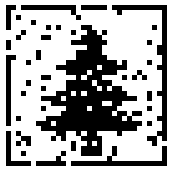
\includegraphics[scale=.4]{image/citizen(awgn).png} \\
  \hline
 Re-sampling & 0.9158 & 10.64 & 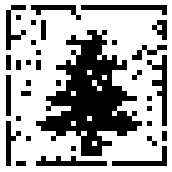
\includegraphics[scale=.4]{image/citizen(resampling).png} \\
  \hline
 Low-pass filtering & 0.9145 & 10.84 & 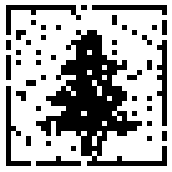
\includegraphics[scale=.4]{image/citizen(lpf).png} \\
  \hline
 Re-quantization & 0.9172 & 10.45 & 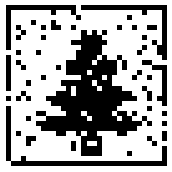
\includegraphics[scale=.4]{image/citizen(requantized).png} \\
 \hline 
 Echo & 0.9268 & 9.28 & 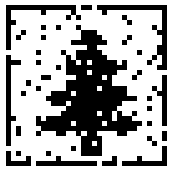
\includegraphics[scale=.4]{image/citizen(echo).png} \\
  \hline
 Reverse & 0.9199 & 10.16 & 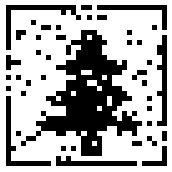
\includegraphics[scale=.4]{image/citizen(reverse).png} \\
  \hline
 mp3 compression (32 kbps) & 0.9225 & 9.77 & 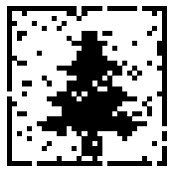
\includegraphics[scale=.4]{image/citizen(32).png} \\
  \hline
 mp3 compression (64 kbps) & 0.9279 & 9.18 & 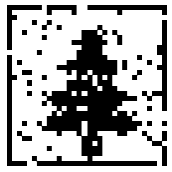
\includegraphics[scale=.4]{image/citizen(64).png} \\
  \hline
 mp3 compression (128 kbps) & 0.9271 & 9.28 & 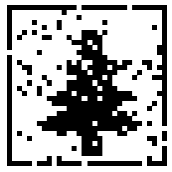
\includegraphics[scale=.4]{image/citizen(128).png} \\
 \hline
 \end{tabular}
 \newline
 \caption{The result of attacks for audio signal (a)}
 \label{table:soundone}
\end{table}



\begin{table}[h!]
 \centering
\begin{tabular}{|c|c|c|c|}
\hline 
Audio Signal & Attack & NC & BER \\ 
\hline 
\multirow{9}{*}{(b) Beginning of the End} 
& Noise addition & 0.9141 & 10.84 \\
\cline{2-4}
& Re-sampling & 0.9172 & 10.45 \\
\cline{2-4}
& Low-pass filtering & 0.9232 & 9.77 \\
\cline{2-4}
& Re-quantization & 0.9262 & 9.38 \\
\cline{2-4}
& Echo & 0.9108 & 11.33 \\
\cline{2-4}
& Reverse & 0.9233 & 9.77 \\
\cline{2-4}
& mp3 compression (32 kbps) & 0.9270 & 9.28 \\
\cline{2-4}
& mp3 compression (64 kbps) & 0.9162 & 10.64 \\
\cline{2-4}
& mp3 compression (128 kbps) & 0.9154 & 10.65 \\
\hline

\multirow{9}{*}{(c) Breathing on Another Planet} 
& Noise addition & 0.9264 & 9.57 \\
\cline{2-4}
& Re-sampling & 0.9129 & 11.04 \\
\cline{2-4}
& Low-pass filtering & 0.9135 & 10.94 \\
\cline{2-4}
& Re-quantization & 0.9228 & 9.77 \\
\cline{2-4}
& Echo & 0.9213 & 9.96 \\
\cline{2-4}
& Reverse & 0.9170 & 10.45 \\
\cline{2-4}
& mp3 compression (32 kbps) & 0.9194 & 10.16 \\
\cline{2-4}
& mp3 compression (64 kbps) & 0.9156 & 10.64 \\
\cline{2-4}
& mp3 compression (128 kbps) & 0.9108 & 11.23 \\
\hline

\multirow{9}{*}{(d) Thousand Yard Stare} 
& Noise addition & 0.9187 & 10.25 \\
\cline{2-4}
& Re-sampling & 0.9194 & 10.26 \\
\cline{2-4}
& Low-pass filtering & 0.9132 & 11.04 \\
\cline{2-4}
& Re-quantization & 0.9214 & 9.96 \\
\cline{2-4}
& Echo & 0.9162 & 10.64 \\
\cline{2-4}
& Reverse & 0.9041 & 12.11 \\
\cline{2-4}
& mp3 compression (32 kbps) & 0.9108 & 11.33 \\
\cline{2-4}
& mp3 compression (64 kbps) & 0.9136 & 10.94 \\
\cline{2-4}
& mp3 compression (128 kbps) & 0.9194 & 10.25 \\
\hline
\end{tabular} 
 \newline
 \caption{The result of attacks for audio signal (b), (c), and (d)}
 \label{table:soundtwo}
\end{table}


\newpage

Tables \ref{table:comparisonNC} and \ref{table:comparisonBER} give the comparative results of proposed scheme with other watermarking schemes for audio \textit{Citizen, Go Back to Sleep} in terms of NC and BER respectively.

\bigskip

Table \ref{table:comparisonNC} compares NC of the proposed algorithm and other algorithms for the audio \textit{Citizen, Go Back to Sleep}. For attack 5 and 6 mentioned in chapter 4 i.e., adding echo and doing the reverse, the proposed scheme clearly shows the best result comparing with other schemes. For attacks of adding noise, low-pass filtering and three different types of mp3 compression, this scheme produces better NC values than \cite{dwt} and \cite{ieee}. Except attack 5 and 6, \cite{energy} clearly indicates that it is better than proposed scheme. But it should be noted that NC values greater than 0.9 indicate its robustness against several attack.

\begin{table}[h!]
 \centering
 \begin{tabular}{|c|c|c|c|c|} 
 \hline 
 \multirow{3}{*}{Attack} & \multicolumn{4}{|c|}{NC} \\
 \cline{2-5}
 & Proposed & \cite{energy} & \cite{dwt} & \cite{ieee} \\ 
 \cline{2-5}
 & DHT & Frame energy & DWT & DWT+DCT \\
 \hline
 Noise addition & 0.9206 & 0.9901 & 0.5870 & 0.6619 \\ 
  \hline
Re-sampling & 0.9158 & 0.9950 & 0.9924 & 0.7847 \\ 
 \hline
Low-pass filtering & 0.9145 & 0.9942 & 0.6272 & 0.5541 \\ 
 \hline
Re-quantization & 0.9172 & 1.0000 & 0.9634 & 0.5454 \\ 
 \hline
Echo & 0.9268 & 0.7559 & 0.5820 & 0.7867 \\ 
 \hline
Reverse & 0.9199 & 0.4904 & 0.5737 & 0.6150 \\ 
 \hline
mp3 compression (32 kbps) & 0.9225 & 0.9591 & 0.5774 & 0.4034 \\ 
 \hline
mp3 compression (64 kbps) & 0.9279 & 0.9650 & 0.5673 & 0.4806 \\ 
 \hline
mp3 compression (128 kbps) & 0.9271 & 0.9650 & 0.5524 & 0.7270 \\ 
 \hline
 \end{tabular}
 \newline
 \caption{Comparison of NC among proposed and other algorithm}
 \label{table:comparisonNC}
\end{table}


Table \ref{table:comparisonBER} compares BER of the proposed algorithm and other algorithms for the audio \textit{Citizen, Go Back to Sleep}. The proposed scheme clearly shows the best result comparing with other schemes for attacks of adding echo and doing reverse operation. For attacks of adding noise, low-pass filtering, and mp3 compression, this scheme produces better NC values than \cite{dwt} and \cite{ieee} but shows comparatively worse result than \cite{energy}. And table \ref{table:comparisonBER} shows that values of \cite{energy} clearly superior to the proposed scheme in term of BER except attack 5 and 6.

\begin{table}[h!]
 \centering
 \begin{tabular}{|c|c|c|c|c|} 
 \hline
 \multirow{3}{*}{Attack} & \multicolumn{4}{|c|}{BER} \\
 \cline{2-5}
 & Proposed & \cite{energy} & \cite{dwt} & \cite{ieee} \\ 
 \cline{2-5}
 & DHT & Frame energy & DWT & DWT+DCT \\
 \hline
 Noise addition & 10.06 & 1.17 & 47.85 & 37.50 \\ 
  \hline
Re-sampling & 10.64 & 0.59 & 0.98 & 25.00 \\ 
 \hline
Low-pass filtering & 10.84 & 0.68 & 43.65 & 50.00 \\ 
 \hline
Re-quantization & 10.45 & 0.00 & 4.69 & 49.00 \\ 
 \hline
Echo & 9.28 & 27.83 & 49.02 & 25.00 \\ 
 \hline
Reverse & 10.16 & 56.64 & 48.63 & 43.75 \\ 
 \hline
mp3 compression (32 kbps) & 9.77 & 4.79 & 49.51 & 62.50 \\ 
 \hline
mp3 compression (64 kbps) & 9.18 & 4.10 & 49.71 & 56.25 \\ 
 \hline
mp3 compression (128 kbps) & 9.28 & 4.10 & 52.25 & 31.25 \\ 
 \hline
 \end{tabular}
 \newline
 \caption{Comparison of BER among proposed and other algorithm}
 \label{table:comparisonBER}
\end{table}

\newpage

\begin{figure}[h!]
\centering
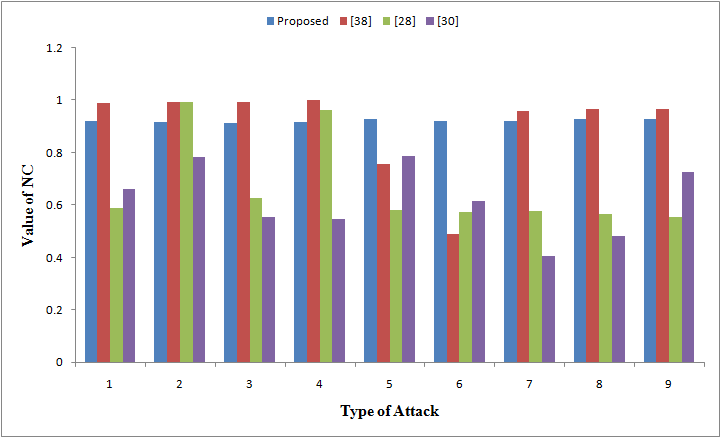
\includegraphics[scale=.7]{image/NC.png}
\caption{Graphical representation of NC comparison}
\label{fig:NC}
\end{figure}

\begin{figure}[h!]
\centering
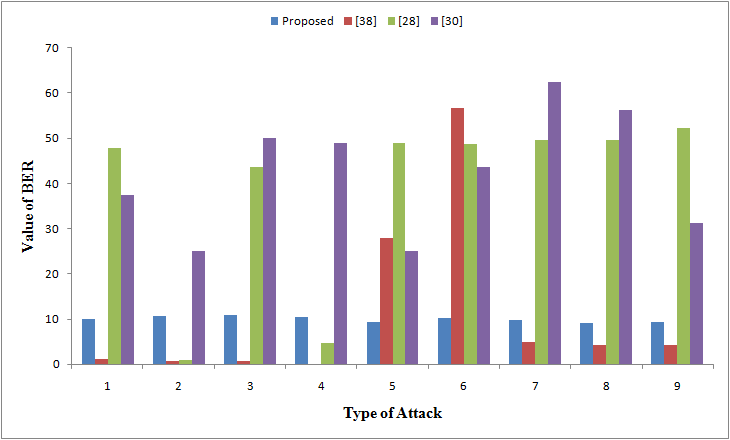
\includegraphics[scale=.7]{image/BER.png}
\caption{Graphical representation of BER comparison}
\label{fig:ber}
\end{figure}

Fig. \ref{fig:NC} and Fig. \ref{fig:ber} show the comparative graphical representation of proposed and other algorithms in terms of NC and BER for table \ref{table:comparisonNC} and \ref{table:comparisonBER} respectively.

\bigskip

Here, each attack is placed on the horizontal axis and value of NC and BER for each attack for different schemes is placed in the vertically against respective attack. From these two graphical charts, it can be easily observed which scheme is better or worse against different attacks. For example, from Fig. \ref{fig:ber}, it can be seen that, for attack number 6, i.e., doing the reverse of audio, proposed scheme produces below 15\% of BER, whereas other three schemes produce above 40\% of BER, which indicates the out-performance of the proposed scheme.

\bigskip

Simulation results indicate that the proposed audio watermarking scheme provides better NC and BER as compared to \cite{dwt}, \cite{ieee} and \cite{energy}. As in this method, there is no need to embeds watermark in the original audio, so it can be said imperceptible, actually the watermarked audio is identical to original one.

\section{False Positive Error}

\begin{figure}[h!]
\centering
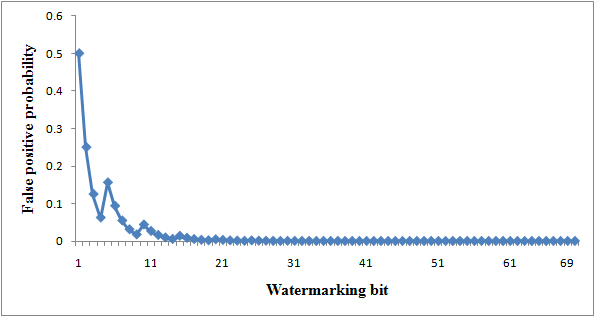
\includegraphics[scale=.8]{image/falsepositive.png}
\caption{False positive probabilities under various watermarking bit}
\label{fig:falsepositive}
\end{figure}

\bigskip

Fig. \ref{fig:falsepositive} gives the false positive probabilities when watermarking bit $(q)$ belongs to $(0, 70]$, and it tells us that the false positive probability trends to $0$ when q is bigger than $14$. In this proposed scheme, $q = 1024$, therefore, the false positive probability is approximately equal to 0.

\bigskip

\section{False Negative Error}

\begin{figure}[h!]
\centering
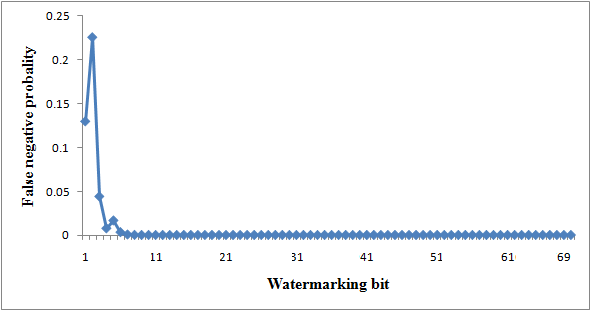
\includegraphics[scale=.8]{image/falsenegative.png}
\caption{False negative probabilities under various watermarking bit}
\label{fig:falsenegative}
\end{figure}

\bigskip

Fig. \ref{fig:falsenegative} gives the false negative probabilities when q belongs to $(0, 70]$, and it tells us that the false rejection probability trends to $0$ when $q$ is bigger than $10$. In this proposed scheme, $q = 1024$, so, the false negative probability of the proposed scheme is also approximately equal to $0$. From tables \ref{table:soundone}, and \ref{table:soundtwo}, it is easily seen that the BERs are all less than $13\%$, so the value of $p$ is assumed to be $0.87$ in this proposed scheme and put this value in equation \ref{eq:falseneg} given at page \pageref{eq:falseneg}.

\chapter{Conclusion}

\section{Summary}

The aim of this thesis was to develop an imperceptible and robust watermarking algorithm that would perform better than existing watermarking methods. For accomplishing this purpose, a new zero-watermarking scheme based on Discrete Hartley Transform has been proposed. Zero-watermarking which does not modify the original audio but constructs zero watermarks from it, is a useful technique for resolving the contradiction between robustness and imperceptibility. The experimental result shows that the proposed watermarking scheme is much better than other. The proposed method provides normalized coefficient (NC) values ranging from 0.90 to 0.92 and also provides bit error rate (BER) values ranging from 9\% to 12\%. Therefore, the proposed scheme provides better robustness against various attacks such as re-sampling, adding echo, compression, etc. Also, the proposed scheme is blind as extracting of the watermark does not require the original signal. Comparison of results with other schemes show that the proposed scheme can be a good competent in the field of audio watermarking.


\section{Future Recommendation}

Since zero-watermarking is a considerably new method and Discrete Hartley Transform (DHT) was not use in the field of audio watermarking, this work offers many opportunities for future work. The followings should consider for the upcoming newer in this field:

\begin{itemize}
\item Other properties of DHT can be considered for getting more robustness.

\item Some modern attacks such as pitch-scale, channel fading, packet drop should be considered.
\end{itemize}

\bibliographystyle{IEEEtran}
\bibliography{IEEEabrv,references}

%\newpage
%
%\appendix

%\begin{appendices}
%
%\chapter{Source Code}
%
%\lstinputlisting{code/attack.m}
%
%\lstinputlisting{code/imageP.m}
%
%\lstinputlisting{code/audioP.m}
%
%\lstinputlisting{code/dht.m}
%
%\lstinputlisting{code/prim.m}
%
%\lstinputlisting{code/bigmod.m}
%
%\lstinputlisting{code/ncber.m}
%
%\end{appendices}

\end{document}
